\documentclass[11pt]{article}
\usepackage[margin=1in]{geometry}
\usepackage{amsmath,amssymb,amsthm}
\usepackage{booktabs}
\usepackage{array}
\newcolumntype{L}[1]{>{\raggedright\arraybackslash}p{#1}}
\usepackage{graphicx}
\usepackage{xcolor}
\usepackage{microtype}
\usepackage[colorlinks=true,linkcolor=blue!50!black,citecolor=blue!50!black,urlcolor=blue!50!black]{hyperref}
\newtheorem{theorem}{Theorem}[section]
\newtheorem{proposition}[theorem]{Proposition}
\newtheorem{lemma}[theorem]{Lemma}
\newtheorem{corollary}[theorem]{Corollary}
\theoremstyle{definition}
\newtheorem{definition}[theorem]{Definition}
\newtheorem{computation}[theorem]{Computation}
\newtheorem{conjecture}[theorem]{Conjecture}
\theoremstyle{remark}
\newtheorem{remark}[theorem]{Remark}
\newtheorem{constraint}[theorem]{Constraint}
\newcommand{\R}{\mathbb R}
\newcommand{\C}{\mathbb C}
\newcommand{\Z}{\mathbb Z}
\newcommand{\F}{\mathbb F}
\newcommand{\Q}{\mathbb Q}
\newcommand{\PA}{\mathrm{PA}}
\newcommand{\ZFC}{\mathrm{ZFC}}
\newcommand{\Con}{\mathrm{Con}}
\newcommand{\Tst}{T^{*}}
\newcommand{\PS}{\mathcal P}
\newcommand{\Hrec}{H_{\mathrm{record}}}
\newcommand{\Ree}{\operatorname{Re}}
\newcommand{\abar}{\bar\alpha}
\title{Across the Horizon\\ \large The running proof, the edge of the cone, the eigenvalues of a curve,\\ and the space on the other side}
\author{Christophe Michaels}
\date{October 5, 2026}
\begin{document}
\maketitle

\begin{abstract}
\noindent This paper joins the running proof of the Michaels programme (the 217-page manuscript of October 4, 2026, Parts 0--XVII, whose single arithmetic target is the subpower growth of the historical Möbius energy) to the work that followed it: the record estimate and the lifetime census, the light cone of the Weil form with its horizon and potential set, the Gödel theorem for the Riemann Hypothesis, and the cone over a curve over a finite field. It does three things. First it locks down where the edge is: in the stones' coordinates the subpower exponent is a statement at infinity, in the rule's coordinates it is the line $\Ree s=\tfrac12$, the fixed set of the reflection $s\mapsto1-\bar s$, and the Mellin transform is the map between the two; every proved equivalence of the programme is a different name for that one edge, and under the Hypothesis the Weil form has no null vector at any finite support, so the edge is reached at no finite half-width. Second it follows the edge through the eigenvalues: the dilation group of the running proof's Part VI is the Berry--Keating operator, the Hypothesis is the reality of its spectrum, the missing piece is an inner product, and on a curve over $\F_q$ every piece exists: Frobenius is the operator, the Lefschetz trace formula turns the stones into traces, unitarity is the Hypothesis, the Hodge index theorem supplies the inner product, and the cone closes at the finite half-width $g\log q$. Third it states what the space on the other side of the horizon must satisfy for $\zeta$ itself, six constraints with their sources in the record, and places the known candidates against them. Nothing here proves the Riemann Hypothesis. Every statement is labelled proved, cited, computed, or conjectured.
\end{abstract}

\tableofcontents

\section*{Status conventions}
A \textbf{Theorem}, \textbf{Proposition} or \textbf{Lemma} without a citation is proved in the text or in the cited document of the programme, where the proof is complete. A statement with a citation to the literature is taken from there with its hypotheses. A \textbf{Computation} is a numerical result with its method and its file in the repository. A \textbf{Constraint} is a proved property that any candidate for the space of Section~\ref{sec:space} must have. A \textbf{Conjecture} is a precise statement with the evidence for and against it, and is never used as a premise.

\section{The stones: the running proof in one page}\label{sec:stones}

The running proof \cite{running} is the active manuscript of the programme. Its earlier chapters are the former 125-page edition restored in full; its later parts are the continuations through October 4, 2026. Its twelve-page companion \cite{summary} states the argument it selects. Everything in this section is quoted from those two documents with their own status.

\subsection{The dictionary}
With $\mu$ the Möbius function,
\[
M(x)=\sum_{n\le x}\mu(n),\qquad I_M(N)=\int_1^N\frac{M(t)^2}{t^2}\,dt,\qquad T(N)=\frac{M(N)^2}{N},\qquad R(N)=I_M(N)+T(N).
\]
$I_M$ is the historical energy, $R$ the native Green energy. The single arithmetic target of the running proof is
\begin{equation}\label{eq:H}\tag{H}
I_M(X)\le C_\varepsilon X^{\varepsilon}\qquad(X\ge2)\quad\text{for every }\varepsilon>0,
\end{equation}
with the quantifiers fixed by \cite[\S2]{summary}: for every $\varepsilon$ one constant works for every $X$. This is what ``subpower'' means. It permits irregular growth, uneven contributions and arbitrarily long individual lifetimes; it is not a condition on any one scale, colour or packet.

\subsection{What is proved}
\begin{theorem}[conditional closing theorem; {\cite[\S11]{summary}}, {\cite[Part 0]{running}}]\label{thm:closing}
\eqref{eq:H} implies that every nontrivial zero of $\zeta$ has real part $\tfrac12$.
\end{theorem}
The proof is the Mellin deduction: \eqref{eq:H} gives weighted absolute integrability of $M$, hence a holomorphic continuation of $s\int_1^\infty M(x)x^{-s-1}dx$ to $\Ree s>\tfrac12$; its agreement with $1/\zeta(s)$ for $\Ree s>1$ excludes zeros in $\Ree s>\tfrac12$; the functional equation excludes them in $\Ree s<\tfrac12$. The converse is classical (Littlewood, \cite[\S14.25]{titchmarsh}): under the Hypothesis $M(x)\ll x^{1/2+\varepsilon}$, hence \eqref{eq:H}. So \eqref{eq:H} is equivalent to the Riemann Hypothesis, and the running proof's own status line says that \eqref{eq:H} is the premise and is not established.

\begin{theorem}[lifetime identity and truncation; {\cite[Part XVII, (NL1)--(NL2)]{running}}]\label{thm:lifetime}
For a level of $|M|$ born at $u$ with depth $h_u$, odd weight $w_u=2h_u-1$ and first closing downcrossing $v_u$ ($=\infty$ if unobserved),
\[
I_M(N)=\sum_{u\le N}w_u\Big(\frac1u-\frac1{\min(v_u,N)}\Big),\qquad
\mathcal E_\star(N)\le I_M(N)\le 2\log N+\mathcal E_\star(N),
\]
where $\mathcal E_\star(N)=\sum w_ud_u/(u(u+d_u))$ over the levels with $w_ud_u>u$ and $d_u=(\min(v_u,N,h_u^2)-u)^+$.
\end{theorem}
So the subpower target is equivalent to the same rate for the retained early lifetime costs $\mathcal E_\star$. The nested multiplicative channels $M=\prod_{p\in S}(I-D_p)A_S$ and the exact overlap formulas (NL3)--(NL6) are proved identities whose sign is not prescribed. The direction retained after consolidation is the sentence on page 217: \emph{the nested structure must explain why expensive lifetimes cannot occur frequently enough, or persist long enough, to violate subpower growth.}

\subsection{What followed}
Three later documents sharpen the target without changing its strength.
\begin{itemize}
\item \textbf{The record estimate} \cite{hrec}. $\Hrec$, the record form of the energy bound, is equivalent to the Hypothesis (Theorem 3.1 there), with the exponent dictionary: $\Hrec(\theta)$ implies no zeros with $\Ree s>\tfrac12+\theta$. The debit identity $\Delta_N=E(u_0)+2M(m)h(u_0)+E(W)-2\langle a,W\rangle$ is exact; the two positive terms are each at least $(1-o(1))\,m/(24\log^2m)$, so no term-by-term bound can give the target and the signed cross term carries the cancellation. The route around $h$ (Section 7 there) removes the history term exactly and returns it as a mean obligation, a square-root bound on $\sum_{m<n\le N}\mu(n)/n$.
\item \textbf{The lifetime census} \cite{census,censusaudit}. The census reformulation, the sliding mean, Landau's one-sided closure, the Buchstab--Dickman comparison and the complete prime-discrepancy residual $\mathcal Z_N$ are exact; every target in it, (9), (S34), (C27), (Z14), (J27), is equivalent to the Hypothesis; every proved credit is below the allowance $N^{1/2+\varepsilon}$, and the paid insertion range is the Legendre range $2^{\pi(Y)}\le\sqrt N$, beyond which the alternating cofactor sum meets Selberg's parity obstruction.
\item \textbf{The Gödel theorem} \cite{gstring}. The Hypothesis is a $\Pi^0_1$ sentence $\rho$ \cite{dmr}; adding every true $\Sigma^0_1$ sentence to $\PA$ or $\ZFC$ adds no theorem, so no verified pattern to any bound proves $\rho$; $\PA\vdash\rho\leftrightarrow\Con(\mathrm Q+\rho)$ and $\ZFC\vdash\rho\leftrightarrow\Con(\PA+\rho)$; any true principle that establishes $\rho$ over $\PA$ is unprovable in $\PA$, not equivalent to any finitely verifiable fact, and proves $\Con(\mathrm Q+\rho)$.
\end{itemize}

\subsection{The one observation this paper adds to Section~\ref{sec:stones}}
\eqref{eq:H} is a statement about the growth exponent at infinity, $\limsup\log I_M(X)/\log X=0$. No finite computation touches it: $I_M(N)$ to any $N$ is a $\Sigma^0_1$ fact and, by the inertness theorem, inert. Every quantity the running proof pays, $2\log N$, the aggregate allowances, the Legendre range, is a quantity the target already tolerates. The subpower is therefore the first object in the programme that is not finitary, and it is the only one. This is not a weakness of the running proof; it is where the Hypothesis sits, and the next section locks that position down.

\section{The edge, locked down}\label{sec:edge}

\subsection{The cone}
For $f$ real with compact support, $g=f\star\tilde f$ and $\hat g=|\hat f|^2$, the Weil form in the normalization of \cite{window,zhu} is
\[
Q(f)=W_\infty(g)-\sum_{n\ge2}\frac{\Lambda(n)}{\sqrt n}\big(g(\log n)+g(-\log n)\big)+\hat g(\tfrac i2)+\hat g(-\tfrac i2)=\sum_\rho\hat g\big(\tfrac{\rho-1/2}{i}\big),
\]
the last equality by the explicit formula \cite{weil52}. For $f$ supported in $[-a,a]$ the autocorrelation $g$ is supported in $[-2a,2a]$, so only the prime powers with $\log n<2a$ enter: this is the light cone of \cite[\S12]{folds}, with half-width $a$ as time, $\log n$ as space, the edge $\log n=2a$, and the entries $a_n=\tfrac12\log n$ at which each prime power switches on. The form $Q$ does not depend on $a$, so the floor
\[
\lambda(a)=\inf\{Q(f):\ f\text{ odd},\ \operatorname{supp}f\subset[-a,a],\ \|f\|_2=1\}
\]
is non-increasing, and it is attained \cite[Lemma 1.4]{window}.

\begin{theorem}[Weil \cite{weil52}; Yoshida \cite{suzuki}]\label{thm:weil}
The Riemann Hypothesis holds if and only if $Q(f)\ge0$ for every compactly supported smooth $f$, and the odd $f$ already suffice. Hence $\mathrm{RH}\iff\lambda(a)\ge0$ for all $a>0$.
\end{theorem}

\begin{theorem}[Zhu {\cite[Thm.\ 6.2]{zhu}}]\label{thm:zhu}
$8.206\times10^{-15}\le\lambda(0.8)\le2.347\times10^{-14}$, certified by interval arithmetic; so $\lambda(a)>0$ for $0<a\le0.8$.
\end{theorem}

\begin{definition}[the horizon]
$\Tst(a)=2\pi e^{2a}$.
\end{definition}
A function of exponential type $a$ has zeros of upper density at most $a/\pi$ on a half-line \cite{boas}; the zeros of $\zeta$ have density $(2\pi)^{-1}\log(t/2\pi)$ at height $t$, which equals $a/\pi$ exactly at $t=\Tst(a)$ \cite[\S1]{window}. The horizon is the height at which the zeros become too dense for the window: below it the minimizer's transform interpolates the zeros, above it the minimizer is exponentially small \cite[Computation 12.5]{folds}. The floor decays with the horizon.

\begin{computation}[the floor; {\cite{folds,window}}, files \texttt{floor\_grid\_K40.csv}, \texttt{floor\_grid\_arb.csv}]\label{comp:floor}
In the odd sector, $\lambda(0.3)=0.2226$, $\lambda(0.549)=1.49\times10^{-5}$, $\lambda(1.2)=7.2\times10^{-37}$ (40 modes), $\lambda(1.505)\in[8.1,11.2]\times10^{-94}$ (certified enclosures, 180--230 modes). The horizon at $a=1.5$ is $\Tst=126$; the floor is positive at every support computed. Prime $2$ enters at $a=0.3466$ and is needed by $a=0.3716$, where the prime-free form turns indefinite; the entries and deadlines of $3,4,5,7,8,9$ are Table 1 of \cite{folds}.
\end{computation}

\subsection{The potential set: the hollow image}
\begin{definition}[{\cite[Def.\ 2.1]{potential}}]
For $a>0$, $\PS(a)$ is the set of positive Radon measures $\nu$ on $\R$, symmetric, with $\int(1+t^2)^{-1}d\nu<\infty$, such that $\int\hat g\,d\nu=\langle W,g\rangle$ for every even $g\in C_c^\infty(-2a,2a)$, where $\langle W,g\rangle$ is the prime-and-archimedean side of the explicit formula. Put $\nu_\zeta=\sum_\rho\delta_{\gamma_\rho}$ when all $\gamma_\rho$ are real.
\end{definition}
An element of $\PS(a)$ is a configuration of zeros that no prime power inside the cone can distinguish from the true one. It is the mold, not the cast: at support $a$ the stones inside the cone do not give the zeros, they give the set of everything the zeros could still be.

\begin{proposition}[{\cite[Props.\ 2.2--2.3]{potential}}]\label{prop:potential}
(i) $\PS(a)$ is non-increasing in $a$. (ii) $\PS(a)\ne\emptyset$ if and only if the Weil form is nonnegative at support $a$ (Krein's extension theorem in distributional form). (iii) $\bigcap_{a>0}\PS(a)=\{\nu_\zeta\}$ if the Hypothesis holds and $=\emptyset$ otherwise.
\end{proposition}
By Theorem~\ref{thm:zhu} and (ii), $\PS(0.8)\ne\emptyset$ unconditionally. As $a\downarrow0$ only the archimedean singularity constrains $\nu$, fixing its large-scale density to the Riemann--von Mangoldt law; each prime power entering at $a_n$ adds one constraint at the frequency $\log n$. The identity prescribes how many zeros there are, the primes prescribe where they are, one frequency at a time, and $\PS(a)$ is what remains open.

\subsection{The edge of the minimizer}
The word ``edge'' has a second, literal meaning in the programme, and it is the mechanism of the decay. Write $f_a$ for the minimizer at support $a$.
\begin{theorem}[the edge law; {\cite[Thm.\ 3.2]{window}} from Chen--Weth \cite{chenweth} and \cite{hls}]\label{thm:edgelaw}
Under the boundedness hypothesis $(\mathrm H_\infty)$ of \cite{window}, $f_a$ is continuous on $\R$, $f_a(\pm a)=0$, and $|f_a(y)|\le C_0(\log\frac1{a-|y|})^{-1/2}$ near the ends. Numerically $f_a(a-\delta)=C\,(\log(a/\delta)+\beta)^{-1/2}(1+o(1))$ with $C=0.0241$, $\beta=-1.87$ at $a_3$ \cite[Computation 3.4]{window}.
\end{theorem}
\begin{theorem}[the boundary law; {\cite[Thm.\ 9.12 and the every-support theorem of \S9]{window}}]\label{thm:boundary}
Let $A_0(a)$ be the edge amplitude of $f_a$. Then $\lambda'(a)=-2|A_0(a)|^2$ at almost every support, and in dilation form $a\lambda'(a)=-[D_\infty(f_a)+D_P(f_a)+2P(f_a)^2+2P(f_a)M(f_a)]$.
\end{theorem}
\begin{theorem}[the reduction; {\cite[Main theorem]{window}}]\label{thm:reduction}
Under $(\mathrm H_\infty)$ and $(\mathrm H_{\mathrm{BV}})$, if $2|A_0(a)|^2\le(c\,\Tst(a)+e(a))\lambda(a)$ for almost every $a\ge a_Z$, with $c$ a constant and $e$ integrable, then $\lambda(a)>0$ for every $a$ and the Riemann Hypothesis holds.
\end{theorem}
The content of the three theorems together: the floor decays only through what the minimizer does at the window's edge, and the Hypothesis is the statement that the edge amplitude never outruns the floor by more than the horizon allows. The inequality contains the Hypothesis, since it fails wherever the floor is negative. The edge of the cone (the line $\log n=2a$) and the edge of the minimizer (the points $y=\pm a$) are the same place seen in the two variables.

\subsection{Where the edge is}
\begin{theorem}[the edge theorem]\label{thm:edge}
The following statements are equivalent, and each equivalence is proved in the cited document:
\begin{enumerate}
\item[(1)] the Riemann Hypothesis;
\item[(2)] the subpower bound \eqref{eq:H} (Theorem~\ref{thm:closing} and Littlewood);
\item[(3)] the record estimate $\Hrec$ \cite[Thm.\ 3.1]{hrec};
\item[(4)] $\lambda(a)\ge0$ for every $a>0$ (Theorem~\ref{thm:weil});
\item[(5)] $\bigcap_a\PS(a)=\{\nu_\zeta\}$ (Proposition~\ref{prop:potential}(iii));
\item[(6)] the residual bound $\mathcal Z_N\ge-C_\varepsilon N^{1/2+\varepsilon}$ of the census \cite[\S62]{census}, and likewise its targets (9), (S34), (C27), (J27);
\item[(7)] over $\ZFC$: $\Con(\PA+\rho)$ \cite[Thm.\ 5.1]{gstring}.
\end{enumerate}
Moreover the exponent version holds: for $0\le\theta<\tfrac12$, the bound $M(x)\ll x^{1/2+\theta+\varepsilon}$ for every $\varepsilon$ implies that every zero satisfies $|\Ree\rho-\tfrac12|\le\theta$, and conversely $\sup_\rho\Ree\rho=\tfrac12+\theta$ implies that bound \cite[\S14.25]{titchmarsh}.
\end{theorem}
\begin{proof}
(1)$\Leftrightarrow$(2): Theorem~\ref{thm:closing} and \cite[\S14.25]{titchmarsh}. (1)$\Leftrightarrow$(3): \cite[Thm.\ 3.1]{hrec}. (1)$\Leftrightarrow$(4): Theorem~\ref{thm:weil}. (1)$\Leftrightarrow$(5): Proposition~\ref{prop:potential}. (1)$\Leftrightarrow$(6): \cite[\S\S4, 26, 62]{census}, checked in \cite[\S4]{censusaudit}. (1)$\Leftrightarrow$(7): \cite[Thm.\ 5.1(iii)]{gstring}. The exponent version: the Mellin deduction of Theorem~\ref{thm:closing} with the abscissa $\tfrac12+\theta$ in place of $\tfrac12$ gives no zeros with $\Ree s>\tfrac12+\theta$, and the functional equation reflects this to $\Ree s<\tfrac12-\theta$; the converse is the classical Perron-formula estimate.
\end{proof}

The exponent version is the reflection stated exactly. A subpower exponent $\theta$ on the stone side is a shell $|\Ree s-\tfrac12|\le\theta$ on the rule side, symmetric because the functional equation reflects $s\mapsto1-\bar s$; the shell is hollow, since the bound says nothing about where inside it the zeros lie; and as $\theta\to0$ the shell closes onto the line, which is the fixed set of the reflection. What is known unconditionally is $\theta=\tfrac12-o(1)$ (Vinogradov--Korobov): the shell is the whole critical strip less a sliver at its two walls. The Hypothesis is that its thickness is zero.

\begin{proposition}[the edge is reached at no finite support]\label{prop:nofinite}
Assume the Riemann Hypothesis. Then for every $a>0$ the Weil form is positive definite on functions supported in $[-a,a]$: $Q(f)=0$ forces $f=0$. In particular $\lambda(a)>0$ for every finite $a$, and the Weil criterion is decided at no finite support.
\end{proposition}
\begin{proof}
Under the Hypothesis $Q(f)=\sum_\rho|\hat f(\gamma_\rho)|^2$ with all $\gamma_\rho$ real. If $Q(f)=0$ then $\hat f$ vanishes at every $\gamma_\rho$. Now $\hat f$ is entire of exponential type at most $a$ and square-integrable on $\R$, so it is in the Cartwright class and has at most $(a/\pi+o(1))T$ zeros of height in $(0,T]$ \cite[Ch.\ 8]{boas}, while $\zeta$ has $(T/2\pi)\log(T/2\pi)+O(T)$ of them. For $T$ large the second exceeds the first unless $\hat f\equiv0$, i.e.\ $f=0$. Since the infimum $\lambda(a)$ is attained \cite[Lemma 1.4]{window}, $\lambda(a)>0$.
\end{proof}

This is the sense in which the edge is at infinity in the stones' coordinates. Over the integers there is no finite half-width at which the form acquires a null vector, no finite support at which the stones inside the cone return the rule, and the collapse of Proposition~\ref{prop:potential}(iii) happens only in the limit. The computed decay of Computation~\ref{comp:floor} is the number-field shadow of a zero the floor never reaches. Section~\ref{sec:eigen} shows the same form reaching zero at a finite support where the object is small enough.

\subsection{Why the edge is at infinity in the logic too}
The Gödel theorem says the same thing in another language, and it is worth saying once in this paper because it explains why the running proof could not have closed by accumulation. $\rho$ is $\Pi^0_1$: $\forall n\,D(n)$ with $D$ decidable \cite{dmr}. Each instance $D(n)$ is a $\Sigma^0_1$ fact and a theorem of Robinson arithmetic; by \cite[Thm.\ 4.1]{gstring} the theory $T+\{\text{all true }\Sigma^0_1\text{ sentences}\}$ has the same theorems as $T$ for every $T\supseteq\mathrm Q$. So every record, every energy to any $N$, every certified floor to any $a$, is inert: it proves nothing that was not already provable. The subpower exponent, the floor's sign at every $a$, the collapse of the potential set, are each the universal sentence, and none of their instances reaches it. The edge is at infinity in the logic for the same reason it is at infinity in Proposition~\ref{prop:nofinite}: the pattern has no last stone.

\section{Through the eigenvalues}\label{sec:eigen}

\subsection{The dilation group is the Berry--Keating operator}
Part VI of the running proof \cite[p.\ 104]{running} records the unitary dilation on $L^2((0,\infty),dx)$,
\[
(U_tf)(x)=e^{t/2}f(e^tx),\qquad U_t\,x^{\rho-1}=e^{(\rho-1/2)t}\,x^{\rho-1},
\]
and notes that a generalized mode $x^{\rho-1}$ is phase-only precisely when $\Ree\rho=\tfrac12$. Its generator is
\[
U_t=e^{itH},\qquad H=-i\Big(x\frac{d}{dx}+\frac12\Big)=\frac{xp+px}{2},\quad p=-i\frac{d}{dx},\qquad H\,x^{\rho-1}=-i\big(\rho-\tfrac12\big)\,x^{\rho-1},
\]
which is the Hamiltonian $xp$ of Berry and Keating \cite{bk}, symmetrized, and the Mellin transform is its spectral representation. For $\rho=\tfrac12+i\gamma$ the eigenvalue is $\gamma$, real exactly when the zero is on the line. This is the Hilbert--Pólya statement \cite{polya}, \emph{the zeros are the eigenvalues of a self-adjoint operator}, with the operator named; and the running proof already records the obstruction in the same paragraph: the modes $x^{\rho-1}$ are not in $L^2$, their norms diverge at one or both ends, so ordinary unitarity cannot be applied to them, and \emph{the useful inherited question is how authentic arithmetic states acquire a controlled positive norm.} That question is the inner product. Connes proved that it is the whole question:
\begin{theorem}[Connes \cite{connes99}]\label{thm:connes}
The Riemann Hypothesis is equivalent to the positivity of the Weil distribution, i.e.\ to the existence of an inner product on the test functions in which the explicit formula is the trace of the action of the idele class group; the zeros then appear as an absorption spectrum, with the sign of the prime terms opposite to that of periodic orbits in the Gutzwiller and Selberg trace formulas.
\end{theorem}
The Weil form $Q$ is that inner product's candidate restricted to compact supports, $\lambda(a)\ge0$ is its positivity at support $a$, and Theorem~\ref{thm:edge}(4) is the statement that the inner product exists. The sign remark is the seventh filter of \cite{routes}: any spectral route must say how it handles it.

\subsection{The quantum statistics}
Montgomery \cite{montgomery} showed, under the Hypothesis and for restricted test functions, that the pair correlation of the zeros is that of the eigenvalues of large random Hermitian matrices (the Gaussian unitary ensemble), and Dyson identified the law; Odlyzko's computations near the $10^{20}$-th zero \cite{odlyzko} confirm it to high precision, including the nearest-neighbour spacing, which is beyond what is proved. The pair-correlation statement itself is now unconditional in its restricted range \cite{routes}. This is the ``strangeness'': the zeros repel each other exactly as the energy levels of a heavy nucleus do, and no operator is known that produces them.

\subsection{The curve: every piece exists}
Let $X/\F_q$ be a smooth projective curve of genus $g$, $N_m=\#X(\F_{q^m})$ its stones, and $b_d$ the number of closed points of degree $d$, so that $N_m=\sum_{d\mid m}d\,b_d$.
\begin{theorem}[Weil \cite{weil48}; trace formula {\cite[Ch.\ VI]{milneEC}}]\label{thm:weilcurve}
There are algebraic integers $\alpha_1,\dots,\alpha_{2g}$, the eigenvalues of Frobenius $F$ on $H^1(X)$, with
\[
N_m=1+q^m-\operatorname{tr}(F^m)=1+q^m-\sum_{i=1}^{2g}\alpha_i^m\qquad(m\ge1),
\]
closed under $\alpha\mapsto q/\alpha$ and under conjugation, and $|\alpha_i|=\sqrt q$ for every $i$.
\end{theorem}
Write $\alpha_i=\sqrt q\,e^{i\theta_i}$, $U=F/\sqrt q$, $H_X=-i\log U$ with eigenvalues $\theta_i$. Then
\[
N_m=1+q^m-q^{m/2}\operatorname{tr}\big(e^{imH_X}\big),
\]
the stones are the quantum trace of a Hamiltonian, and $|\alpha_i|=\sqrt q$ says that $U$ is unitary, that $H_X$ is self-adjoint, that the zeros of $\zeta_X(s)=Z(q^{-s})$ have $\Ree s=\tfrac12$. The inner product is Weil's: the Rosati involution on the endomorphisms of the Jacobian is positive, equivalently the Hodge index theorem on $X\times X$ holds, and that positivity is the proof. For $g=1$ it is Hasse's: the degree of an endomorphism is a nonnegative integer, so $\deg(m-nF)=m^2-a_1mn+qn^2\ge0$ for all integers $m,n$, so $a_1^2\le4q$ \cite[Ch.\ V]{silverman}; the stones are the degrees $N_m=\deg(1-F^m)$, and the positivity that forces the circle lives on maps that are not Frobenius powers at all \cite{reading}.

\begin{theorem}[the cone over a curve; {\cite[\S2]{ffcone}}]\label{thm:ffcone}
With $z_i=\alpha_i/\sqrt q$ distinct, $\hat\nu_X(m)=\sum_ie^{im\theta_i}=q^{m/2}+q^{-m/2}-N_mq^{-m/2}$, and $T_{2D+1}=[\hat\nu_X(j-k)]_{|j|,|k|\le D}$ the matrix of the Weil form at support $D$ (half-width $a=D\log q$, closed points of degree $\le2D$ inside the cone):
\begin{enumerate}
\item[(i)] $T_{2D+1}$ is positive definite for $D<g$: the cone is open and the potential set $\PS_X(D)$ is infinite;
\item[(ii)] $T_{2D+1}$ is singular for every $D\ge g$, with null vector the coefficients of $\prod_i(w-\bar z_i)$; hence $\lambda(D)=0$, $\PS_X(D)=\{\nu_X\}$, and the stones $N_1,\dots,N_{2g}$ inside the cone return the zeros: the cone closes at $a=g\log q$;
\item[(iii)] the even sector closes at $D=g$, the odd sector at $D=g+1$;
\item[(iv)] for any $2g$-multiset closed under $z\mapsto\bar z$ and $z\mapsto1/\bar z$, $T_{2g+1}\succeq0$ if and only if every $|z_i|=1$: positivity at the single support $D=g$ is the Riemann Hypothesis for $X$, and an impostor pair off the circle is rejected at some $D\le g$.
\end{enumerate}
\end{theorem}
\begin{computation}[{\cite[\S3]{ffcone}}, files \texttt{data/ff\_cone\_*.json}]
On five hyperelliptic curves (genus $1,2,3$ over $\F_3$, genus $2,3$ over $\F_5$) the functional equation, $|\alpha_i|=\sqrt q$, the counted $\hat\nu_X$ against the zeros, and the explicit formula all check to $10^{-14}$; the even floor is exactly zero at $D=g$ and the odd at $D=g+1$ in every case; the null vector at $D=g$ returns the zeros to $10^{-15}$; every impostor is caught by $D\le g$. For $y^2=x^3+x^2+1$ over $\F_3$ the whole computation is done by hand in \cite{reading}: $N_1=6$, $N_2=12$, $a_1=-2$, $\alpha=-1\pm i\sqrt2$, the $3\times3$ form at $a=\log3$ has eigenvalues $0,\tfrac83,\tfrac{10}3$, and its null vector $(1,2/\sqrt3,1)$ has roots at $\cos\theta=-1/\sqrt3$, the two zeros.
\end{computation}

\subsection{The statistics on the curve}
Katz and Sarnak \cite{katzsarnak} proved that over families of curves over $\F_q$, as $q\to\infty$, the Frobenius angles $\theta_i$ are distributed as the eigenangles of random unitary (or symplectic, or orthogonal) matrices: the random-matrix law that is conjectural for $\zeta$ is a theorem on the curved plane. Every piece of Section~\ref{sec:eigen} exists on a curve: the operator, the trace formula, the inner product, the unitarity, the statistics, and the closing of the cone at finite support.

\subsection{The dictionary}
\begin{center}
\begin{tabular}{L{0.46\textwidth}L{0.46\textwidth}}
\toprule
curve $X/\F_q$ of genus $g$ & the integers\\
\midrule
closed points of degree $d$ at $d\log q$, weight $d$ & prime powers $n$ at $\log n$, weight $\Lambda(n)$\\
stones $N_1,N_2,\dots$ & $\psi(x)$, $M(x)$, $I_M(N)$\\
rule: $2g$ eigenvalues, one matrix $F$ & rule: infinitely many zeros, no operator known\\
$N_m=1+q^m-q^{m/2}\operatorname{tr}e^{imH_X}$ & $\psi(x)=x-\sum_\rho x^\rho/\rho-\dots$\\
$\mathrm{RH}_X\iff U=F/\sqrt q$ unitary & $\mathrm{RH}\iff$ spectrum of $H$ real (Hilbert--Pólya)\\
inner product: Rosati, Hodge index on $X\times X$ & inner product: positivity of the Weil distribution (Connes)\\
cone closes at $a=g\log q$; floor exactly $0$ & cone never closes; floor $>0$ at every finite $a$ (Prop.~\ref{prop:nofinite})\\
null vector at the horizon returns the zeros & no null vector at any finite support\\
positivity at one support $D=g$ is $\mathrm{RH}_X$ & no finite support decides $\mathrm{RH}$\\
random-matrix statistics proved (Katz--Sarnak) & conjectured, confirmed numerically (Montgomery, Odlyzko)\\
$\mathrm{RH}_X$ for one curve is a finite check & $\rho$ is $\Pi^0_1$ with no last instance\\
\bottomrule
\end{tabular}
\end{center}

\begin{center}
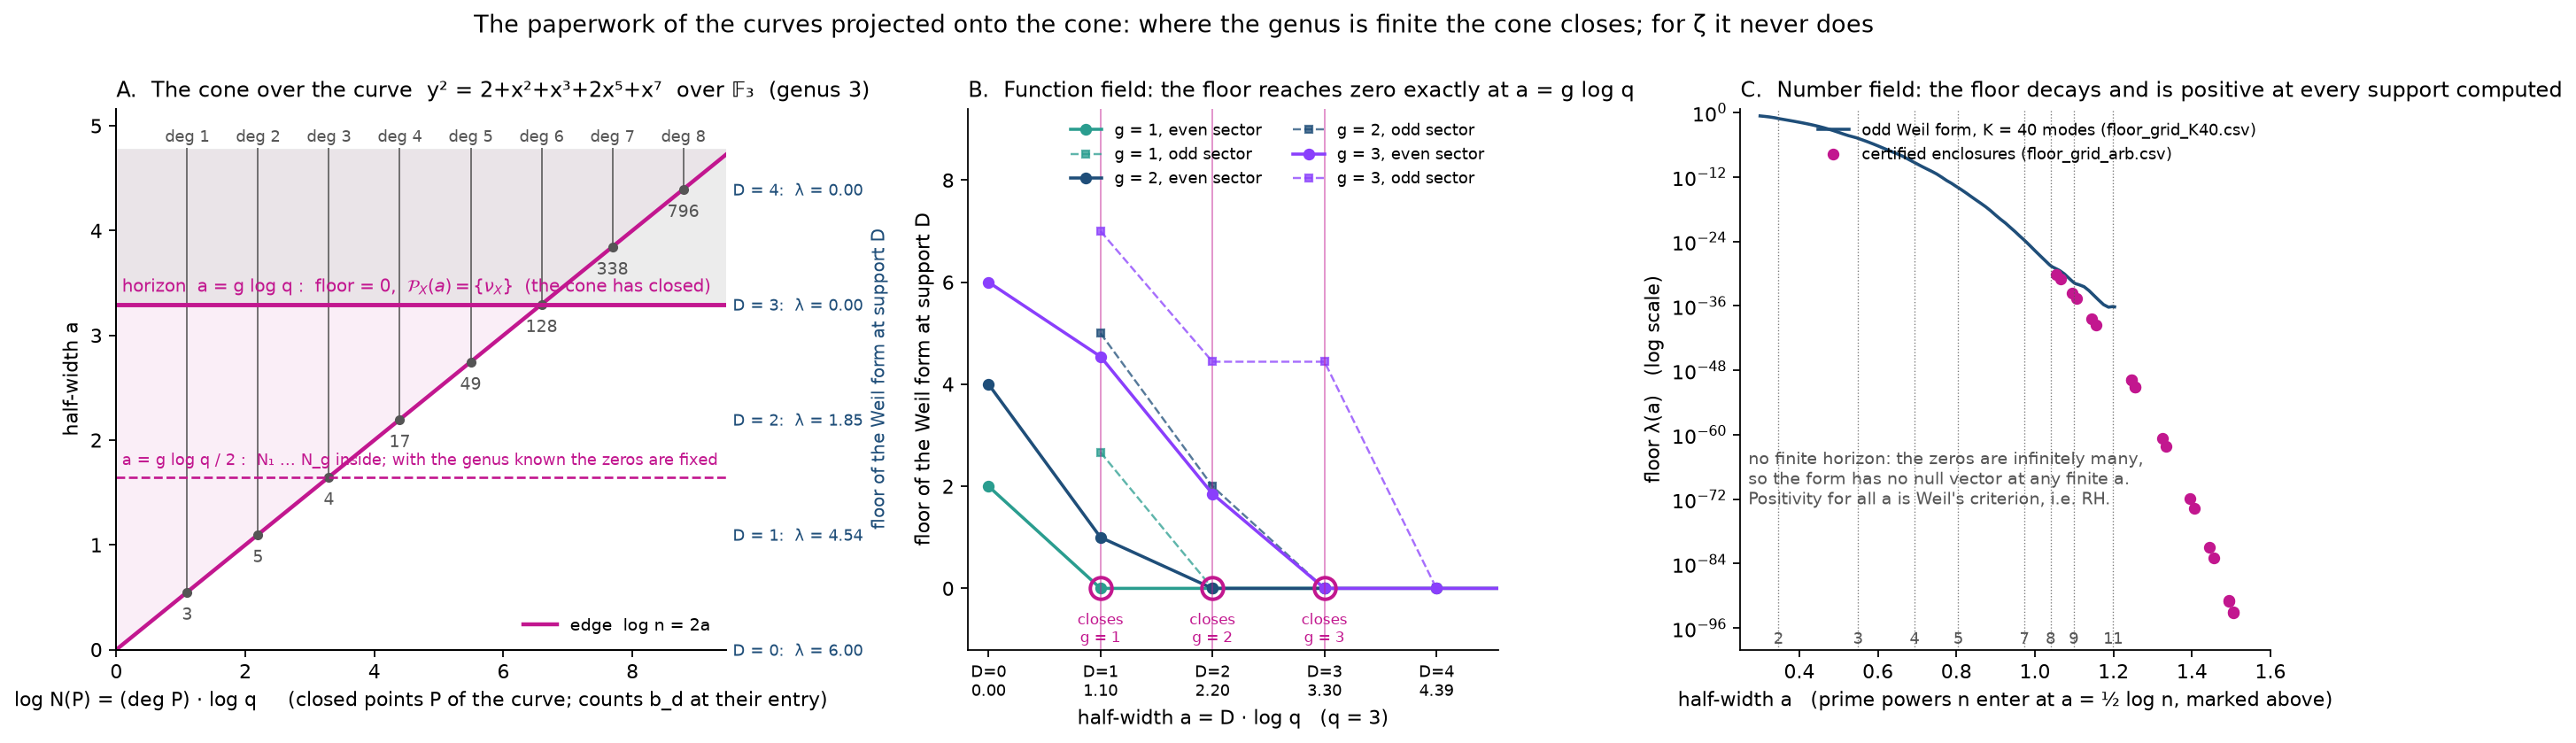
\includegraphics[width=\textwidth]{FUNCTION_FIELD_CONE.png}
\end{center}
\noindent\emph{The cone over the genus-3 curve over $\F_3$, the floors of three curves reaching zero at $g\log q$, and the number-field floor decaying and never reaching zero} (\texttt{FUNCTION\_FIELD\_CONE.png}).

\section{Into the space: what the other side must be}\label{sec:space}

The running proof ends at the subpower; the edge theorem says every road of the programme ends at the same place; the curve shows what lies across the horizon when the object is finite: a space with an operator whose trace is the stones and whose inner product is the Hypothesis. This section states what the corresponding space for $\zeta$ must satisfy. Each constraint is a proved statement with its source; together they are a specification, not a construction.

\begin{constraint}[trace]\label{c:trace}
The explicit formula must be the trace of a flow or operator on the space, with the prime terms entering with their actual sign. (Source: Theorem~\ref{thm:connes} and the sign filter of \cite{routes}; on a curve, the Lefschetz formula $N_m=\sum_i(-1)^i\operatorname{tr}(F^m\mid H^i)$ places the zeros in $H^1$ with the sign $-1$, which is the sign the explicit formula needs.)
\end{constraint}

\begin{constraint}[positivity]\label{c:pos}
The space must carry an inner product in which the trace is a positive form, and that positivity must be equivalent to the Hypothesis. (Source: Theorems~\ref{thm:weil}, \ref{thm:connes}. The floor $\lambda(a)$ is this positivity at support $a$; Theorem~\ref{thm:zhu} certifies it to $a=0.8$, Computation~\ref{comp:floor} observes it to $a=1.5$.)
\end{constraint}

\begin{constraint}[infinite genus]\label{c:dim}
The space is infinite-dimensional, with the dimension of its ``$H^1$ below height $T$'' growing like $N(T)=\frac T{2\pi}\log\frac T{2\pi}+O(T)$, so that the cone of half-width $a$ resolves it only to the horizon $\Tst(a)$ and closes at no finite $a$. (Source: Proposition~\ref{prop:nofinite} and its proof; on a curve the dimension is $2g$ and the cone closes at $a=g\log q$, Theorem~\ref{thm:ffcone}.)
\end{constraint}

\begin{constraint}[entries are orbit lengths]\label{c:orbits}
If the space carries a flow, the entries $a_n=\tfrac12\log n$ of the cone are the half-lengths of its closed orbits: the cone at half-width $a$ sees exactly the orbits of length less than $2a$, and the edge $\log n=2a$ is the orbit-length cutoff. (Source: the explicit formula; the cone of \cite[\S12]{folds}; Deninger's dictionary \cite{deninger}, in which the closed orbits of length $\log p$ are the primes. On a curve the orbits are the closed points, of length $d\log q$.)
\end{constraint}

\begin{constraint}[the axiom from above]\label{c:godel}
Any true principle $\Phi$ about the space from which $\rho$ follows over $\PA$ is unprovable in $\PA$, is not $\PA$-equivalent to any $\Sigma^0_1$ sentence, and proves $\Con(\mathrm Q+\rho)$; if $\rho$ is not provable in $\ZFC$, then $\Phi$ is a new axiom of universal form. (Source: \cite[Thm.\ 6.1, Thm.\ 10.2]{gstring}. On a curve the corresponding principle, Weil's positivity, is a theorem of $\ZFC$, and $\mathrm{RH}_X$ for a single curve is a finite check: the constraint bites only where the pattern has no last stone.)
\end{constraint}

\begin{constraint}[the function-field template]\label{c:template}
The space must reduce, for a curve over $\F_q$, to $H^1(X)$ with Frobenius, and its positivity to the Hodge index theorem on $X\times X$: what must be replaced is the finite dimension $2g$ by the growth of Constraint~\ref{c:dim}, Frobenius by a flow with orbit lengths $\log p$ (Constraint~\ref{c:orbits}), and the surface $X\times X$ by an object whose intersection positivity is Constraint~\ref{c:pos}. (Source: the dictionary of Section~\ref{sec:eigen} and the third filter of \cite{routes}, which asks of every route whether it specializes to curves.)
\end{constraint}

\subsection{The candidates against the constraints}
What follows is the assessment of \cite{routes}, placed against the six constraints; the ranks are those of that document.
\begin{itemize}
\item \textbf{Deninger's foliated dynamical systems} \cite{deninger}. A conjectural cohomology carrying a flow $\phi^t$ with periodic orbits of length $\log p$ (Constraint~\ref{c:orbits}), an infinite-dimensional $H^1$ (Constraint~\ref{c:dim}), the explicit formula as a Lefschetz formula with the right sign (Constraint~\ref{c:trace}), and the Hypothesis as a Kähler-type positivity (Constraints~\ref{c:pos}, \ref{c:template}). This is the picture of Section~\ref{sec:space} stated in 1998 from the cohomology side; the space has not been constructed.
\item \textbf{Connes' adelic trace formula and the arithmetic site} \cite{connes99,cc16}. The trace is proved (Constraint~\ref{c:trace}), the zeros appear as an absorption spectrum with the sign handled, Riemann--Roch for the compactified $\operatorname{Spec}\Z$ is done; the missing step is the positivity (Constraint~\ref{c:pos}), and the authors' own next step is a Hodge-index analogue (Constraint~\ref{c:template}).
\item \textbf{Zeta spectral triples and ground states} \cite{ccm25,cvs25}. Self-adjoint perturbations of scaling operators whose spectra approach the zeros numerically, convergence being equivalent to the Hypothesis; and the theorem that a simple isolated ground state of such a form with an \emph{even} eigenfunction has a transform with only real zeros. The programme works in the odd sector; the odd analogue is open (route 6 of \cite{routes}).
\item \textbf{Berry--Keating and Sierra's models} \cite{bk}. The operator of Section~\ref{sec:eigen} reproduces the smooth zero count $N(T)$ (Constraint~\ref{c:dim}) but not the zeros; the fluctuating part would have to be derived, and the sign filter applies.
\item \textbf{$\F_1$-geometry} (Soulé, Borger, Lorscheid, Durov, Kapranov--Smirnov, Manin; \cite{routes}, route 59). Aims at Constraint~\ref{c:template} directly; none yet gives a cohomology of the size of Constraint~\ref{c:dim}.
\end{itemize}

\subsection{What the record adds to the search}
\begin{enumerate}
\item \textbf{The calibration.} The potential set and the cone are now drawn for both objects with the same coordinate $a$, and they differ in exactly one feature, the finite horizon $g\log q$ (Theorem~\ref{thm:ffcone}, Proposition~\ref{prop:nofinite}). A candidate space can be tested by whether its truncations at support $a$ reproduce the hollow image $\PS(a)$ and never close it.
\item \textbf{The edge law.} The floor's decay is driven at the window's edge (Theorems~\ref{thm:edgelaw}--\ref{thm:reduction}); in a space with a flow the edge is the orbit-length cutoff (Constraint~\ref{c:orbits}). The reduction inequality $2|A_0|^2\le(c\Tst+e)\lambda$ is a statement a candidate space would have to make true: the amplitude at the cutoff against the mass of the spectrum below the horizon.
\item \textbf{The finite-support criterion.} On a curve, positivity at the one support $D=g$ is the Hypothesis (Theorem~\ref{thm:ffcone}(iv)). Proposition~\ref{prop:nofinite} shows that no such support exists for $\zeta$. Any candidate that decides the Hypothesis at a finite truncation is therefore wrong, and any argument that claims to is not about $\zeta$.
\item \textbf{The form of the axiom.} Constraint~\ref{c:godel} says what kind of statement the space's positivity must be: universal, unprovable from the stones, stronger than the consistency of arithmetic with the Hypothesis. The search is for a theorem of this form, and the Gödel theorem says it cannot be reached from below.
\item \textbf{The hollow image.} The potential set is the record's name for what every candidate must reproduce at finite support: not the zeros but the set of configurations the stones leave open, shrinking by one frequency at each entry and never to a point.
\end{enumerate}

\subsection{The human form}
\emph{The Grammar of Things} \cite{grammar} says, in the language of a circle of stones, what Section~\ref{sec:space} says in the language of a space: the records and the rule are two descriptions of one object, neither derivable from the other, and a billion stones perfectly placed honor the rule without moving one inch closer to it, because the distance between them is a border between jurisdictions, not a distance that accumulation crosses. The running proof is the stones placed well. The edge theorem is the border located. The curve is the one case where the border is at a finite distance, because the stones run out. The space on the other side is what the rule is made of.

\subsection{The conjecture}
\begin{conjecture}[Michaels; {\cite[\S10]{gstring}}]\label{conj}
$\rho$ is not provable in $\ZFC$.
\end{conjecture}
\begin{theorem}[{\cite[Thm.\ 10.2]{gstring}}]
If Conjecture~\ref{conj} holds, then the Riemann Hypothesis is true, every instance $D(n)$ and every bounded pattern is provable, $\rho$ is independent of $\ZFC$, and every principle establishing it, in particular the positivity of the space of Section~\ref{sec:space}, is a new universal axiom proving $\Con(\PA+\rho)$.
\end{theorem}
In the terms of this paper: the space exists, its positivity is true, and the positivity is an axiom from above rather than a theorem from below. Evidence for: every road of the programme ends at the same signed comparison; the parity obstruction; the inertness theorem; the structure of the known candidates, each stalled at exactly the positivity step. Evidence against: none is known, and none is known for independence either; no proof, no refutation, no independence result exists. The conjecture is labelled a conjecture, and nothing in this paper depends on it.

\section{Status}\label{sec:status}
\begin{center}\footnotesize
\begin{tabular}{L{0.52\textwidth}L{0.2\textwidth}L{0.2\textwidth}}
\toprule
statement & status & source\\
\midrule
\eqref{eq:H} $\Rightarrow$ RH, and RH $\Rightarrow$ \eqref{eq:H} & proved & Thm.~\ref{thm:closing}, \cite{titchmarsh}\\
lifetime identity and truncation $\mathcal E_\star\le I_M\le2\log N+\mathcal E_\star$ & proved & Thm.~\ref{thm:lifetime}\\
the subpower premise \eqref{eq:H} itself & \textbf{open} & \cite{running,summary}\\
$\Hrec\iff$ RH; exponent dictionary & proved & \cite{hrec}\\
census targets each $\iff$ RH; credits below allowance & proved & \cite{census,censusaudit}\\
Weil's criterion, odd sector & cited & \cite{weil52,suzuki}\\
$\lambda(0.8)>0$ certified & cited & \cite{zhu}\\
floor decay to $a=1.5$, horizon $\Tst=126$ & computed & Comp.~\ref{comp:floor}\\
potential set: monotone, nonempty iff positive, collapse iff RH & proved & \cite{potential}\\
edge law, boundary law, reduction & proved under $(\mathrm H_\infty)$, $(\mathrm H_{\mathrm{BV}})$ & \cite{window}\\
the edge theorem (seven equivalent forms) & proved & Thm.~\ref{thm:edge}\\
no null vector at finite support under RH & proved & Prop.~\ref{prop:nofinite}\\
inertness; $\rho\leftrightarrow\Con(\mathrm Q+\rho)$; closing principle & proved & \cite{gstring}\\
dilation group $=$ Berry--Keating operator; spectrum real iff RH & proved (elementary) & \S\ref{sec:eigen}\\
RH $\iff$ positivity of the Weil distribution (trace form) & cited & \cite{connes99}\\
GUE pair correlation (restricted range) & cited & \cite{montgomery}\\
Weil's theorem for curves; trace formula & cited & \cite{weil48,milneEC}\\
the cone over a curve closes at $a=g\log q$; finite-support criterion & proved & \cite{ffcone}, Thm.~\ref{thm:ffcone}\\
five curves computed; genus-1 case by hand & computed & \cite{ffcone,reading}\\
Katz--Sarnak statistics over families & cited & \cite{katzsarnak}\\
Constraints~\ref{c:trace}--\ref{c:template} & proved, for any candidate & \S\ref{sec:space}\\
the space itself & \textbf{not constructed} & \cite{deninger,cc16}\\
the Michaels Conjecture & conjecture & \cite{gstring}\\
the Riemann Hypothesis & \textbf{open} & \\
\bottomrule
\end{tabular}
\end{center}

\begin{thebibliography}{99}\small
\bibitem{running} C.~Michaels, \emph{Michaels Unified Running Proof: complete continuing manuscript, direct energy argument, and current nested-lifetime research}, Parts 0--XVII (217 pages), consolidated October 4, 2026; the opening volume of \emph{Michaels Unified Proof Manuscript}, this repository (commit 5e9e0dc3).
\bibitem{summary} C.~Michaels, \emph{Direct Historical-Energy Argument: a focused twelve-page conditional proof and current research checkpoint}, October 4, 2026, in \cite{running}, pp.\ 222--233.
\bibitem{hrec} C.~Michaels, \emph{The record estimate $\Hrec$: exact structure, equivalence with the Riemann Hypothesis, and the obstruction in the prime-side expression}, \texttt{RESEARCH\_H\_RECORD.pdf}, October 3, 2026.
\bibitem{census} C.~Michaels, \emph{Lifetime Census and Closing Consequences} (87 pages, \S\S1--73) and \emph{The Complete Residual and a Fictional Closing Mechanism} (\S\S52--73), October 5, 2026, \texttt{received/}.
\bibitem{censusaudit} \emph{Audit of the Lifetime Census and the Complete Residual documents}, \texttt{RESEARCH\_CENSUS\_AUDIT.md}, October 5, 2026.
\bibitem{folds} C.~Michaels, \emph{Primes, Folds, and the One Dot: a computational atlas of Weil positivity, prime-sieve geometry and the zeta zeros}, draft of September 28, 2026, \S12 and Figure 29.
\bibitem{window} C.~Michaels, \emph{Prime DNA: The Floor of the Weil Form}, \texttt{weil\_window.pdf}, October 1, 2026.
\bibitem{potential} C.~Michaels, \emph{The potential set of the light cone}, \texttt{atlas\_potential\_set.pdf}, September 29, 2026.
\bibitem{gstring} C.~Michaels, \emph{RH on a G String: a Gödel theorem for the Riemann Hypothesis}, \texttt{RH\_GODEL\_THEOREM.pdf}, October 5, 2026.
\bibitem{ffcone} \emph{The cone over a curve}, \texttt{FUNCTION\_FIELD\_CONE.md}, October 5, 2026.
\bibitem{reading} \emph{Reading the curve: the stones, the rule and the cone, worked by hand on one curve of genus one}, \texttt{READING\_THE\_CURVE.pdf}, October 5, 2026.
\bibitem{routes} \emph{100 Routes Toward the Riemann Hypothesis, Ranked by Credibility}, \texttt{RH\_ROUTES.md}, September 29, 2026.
\bibitem{grammar} C.~Michaels, \emph{The Grammar of Things}, July 2026, pp.\ 33--35, 70--71, 120, 165--168.
\bibitem{weil52} A.~Weil, Sur les ``formules explicites'' de la th\'eorie des nombres premiers, \emph{Comm. S\'em. Math. Univ. Lund} (1952), 252--265.
\bibitem{suzuki} H.~Yoshida, On Hermitian forms attached to zeta functions, in \emph{Zeta Functions in Geometry}, Adv. Stud. Pure Math. 21 (1992), 281--325; M.~Suzuki, Weil's quadratic form via the screw function, arXiv:2606.09096 (2026).
\bibitem{zhu} X.~Zhu, Weil positivity in compact windows: a finite reduction, certified two-sided bounds, and a Landau--Widom decay law, arXiv:2608.24827 (2026), Theorem 6.2.
\bibitem{boas} R.~P.~Boas, \emph{Entire Functions}, Academic Press, 1954, Ch.\ 8 (Cartwright--Levinson).
\bibitem{chenweth} H.~Chen and T.~Weth, The Dirichlet problem for the logarithmic Laplacian, \emph{Comm. PDE} 44 (2019), 1100--1139.
\bibitem{hls} V.~Hern\'andez-Santamar\'ia, L.~F.~L\'opez R\'ios and A.~Salda\~na, Optimal boundary regularity and a Hopf-type lemma for Dirichlet problems involving the logarithmic Laplacian, \emph{Discrete Contin. Dyn. Syst.} 45 (2025), 1--36.
\bibitem{titchmarsh} E.~C.~Titchmarsh, \emph{The Theory of the Riemann Zeta-Function}, 2nd ed., Oxford, 1986, \S14.25.
\bibitem{dmr} M.~Davis, Y.~Matijasevi\v c and J.~Robinson, Hilbert's tenth problem: Diophantine equations: positive aspects of a negative solution, \emph{Proc. Symp. Pure Math.} 28 (1976), 323--378.
\bibitem{polya} A.~M.~Odlyzko, correspondence with G.~P\'olya on the Hilbert--P\'olya conjecture (1981--82), \texttt{dtc.umn.edu/\textasciitilde odlyzko/polya}.
\bibitem{bk} M.~V.~Berry and J.~P.~Keating, $H=xp$ and the Riemann zeros, in \emph{Supersymmetry and Trace Formulae}, Plenum, 1999, 355--367; The Riemann zeros and eigenvalue asymptotics, \emph{SIAM Review} 41 (1999), 236--266.
\bibitem{connes99} A.~Connes, Trace formula in noncommutative geometry and the zeros of the Riemann zeta function, \emph{Selecta Math.} 5 (1999), 29--106.
\bibitem{cc16} A.~Connes and C.~Consani, Geometry of the arithmetic site, \emph{Adv. Math.} 291 (2016), 274--329.
\bibitem{ccm25} A.~Connes, C.~Consani and H.~Moscovici, zeta spectral triples, arXiv:2511.22755.
\bibitem{cvs25} A.~Connes and W.~D.~van Suijlekom, real zeros of even ground states, arXiv:2511.23257, \emph{Comm. Math. Phys.} (2025).
\bibitem{montgomery} H.~L.~Montgomery, The pair correlation of zeros of the zeta function, \emph{Proc. Symp. Pure Math.} 24 (1973), 181--193.
\bibitem{odlyzko} A.~M.~Odlyzko, On the distribution of spacings between zeros of the zeta function, \emph{Math. Comp.} 48 (1987), 273--308.
\bibitem{katzsarnak} N.~M.~Katz and P.~Sarnak, \emph{Random Matrices, Frobenius Eigenvalues, and Monodromy}, AMS Colloquium Publ.\ 45, 1999; Zeroes of zeta functions and symmetry, \emph{Bull. AMS} 36 (1999), 1--26.
\bibitem{deninger} C.~Deninger, Some analogies between number theory and dynamical systems on foliated spaces, \emph{Doc. Math.} Extra Vol.\ ICM I (1998), 163--186.
\bibitem{weil48} A.~Weil, \emph{Sur les courbes alg\'ebriques et les vari\'et\'es qui s'en d\'eduisent}, Hermann, 1948.
\bibitem{milneEC} J.~S.~Milne, \emph{Lectures on \'Etale Cohomology}, Ch.\ VI (the trace formula); and The Riemann hypothesis over finite fields from Weil to the present day, 2016.
\bibitem{silverman} J.~H.~Silverman, \emph{The Arithmetic of Elliptic Curves}, 2nd ed., Springer, 2009, Ch.\ V.
\end{thebibliography}
\end{document}
